% ch3.tex
% Dieses Werk ist unter einem Creative Commons Namensnennung-Keine kommerzielle Nutzung-Weitergabe
% unter gleichen Bedingungen 3.0 Deutschland Lizenzvertrag lizenziert. Um die Lizenz anzusehen, gehen Sie bitte
% zu http://creativecommons.org/licenses/by-nc-sa/3.0/de/ oder schicken Sie einen Brief an
% Creative Commons, 171 Second Street, Suite 300, San Francisco, California 94105, USA.


%\chapter{Turtles, and other slow moving creatures}\index{turtle}\label{ch:turtles}
\chapter{Schildkröten und andere langsamen Lebewesen}\index{Schildkröte}\label{ch:turtles}

%There are certain similarities between turtles in the real world and a Python turtle.  In the real world, a turtle is a (sometimes) green reptile that moves around very slowly and carries its house on its back.  In the world of Python, a turtle is a small black arrow that moves very slowly around the screen. No mention of house-carrying though.
Es gibt bestimmte Gemeinsamkeiten zwischen einer lebendigen Schildkröte und einer Python Schildkröte. Im echten Leben sind Schildkröten (manchmal) grüne Reptilien, die sich langsam bewegen und ihr Haus auf dem Rücken tragen. In der Python Welt sind Schildkröten schwarze Pfeile die sich sehr langsam am Bildschirm bewegen. Ohne Haus.

%In fact, considering that a Python turtle leaves a trail as it moves around the screen, this makes it less like a real turtle, and more like a snail or a slug.  However, I suppose that a module called `slug' wouldn't be particularly attractive, so it makes sense to stick with turtles.  Just imagine the turtle is carrying a couple of marker pens with it, and drawing as it goes.
Wenn man bedenkt, dass die Python Schildkröte eine Spur am Bildschirm hinterlässt, was für echte Schildkröten ungewöhnlich ist, müsste das Python Modul eher `Nacktschnecke' heißen. Das klingt aber wenig attraktiv und so bleiben wir beim Namen Schildkröte (auf Englisch: turtle). Stell dir einfach vor, dass die Schildkröte ein paar Textmarker mitgenommen hat um ihren Weg zu markieren.

%In the deep, dark, and distant past, there was a simple programming language called Logo.  Logo was used to control a robot turtle (called Irving).  Over time, the turtle evolved from a robot that could move around the floor, to a small arrow moving around a screen.
In der fernen Vergangenheit gab es einmal eine einfache Programmiersprache die Logo genannt wurde. Logo wurde verwendet um eine kleine Roboterschildkröte (mit dem Namen Irving) zu steuern. Die Zeit verging und aus dem Roboter, der sich am Boden bewegte wurde ein kleiner Pfleil am Monitor der sich bewegte.

%\emph{Which just goes to show, things don't always improve as technology advances---a little robot turtle would be a lot more fun.}
\emph{Da kann man sehen, dass die Dinge mit der Zeit nicht immer besser werden. Eine kleine Roboterschildkröte wäre viel lustiger.}

%Python's turtle module (we'll come to modules a bit later, but for now just just think of a module as something we can use inside a program) is a little bit like the Logo programming language, but while Logo was (is) fairly limited, Python has many more capabilities.  The turtle module itself, is a useful way to learn how computers draw pictures on your computer screen.
Das Python Schildkrötenmodul (wir kommen ein wenig später zu Modulen, aber fürs Erste reicht es zu wissen, dass man Module innerhalb von Programmen verwenden kann) ist der Programmiersprache Logo ähnlich. Aber während Logo recht eingeschränkt ist, hat Python sehr viele Möglichkeiten. Mit dem Schildkrötenmodul kann man aber zeigen, wie Computer Bilder auf dem Bildschirm zeichnen.

%Let's get started and see just how it works.  The first step is to tell Python we want to use turtle, by importing the module:
Fangen wir an. Zuerst sagen wir Python, dass wir dieses Schildkrötenmodul verwenden wollen und importieren es:


\begin{Verbatim}[frame=single]
>>> import turtle
\end{Verbatim}

%Then we need to display a canvas to draw on.  A canvas is just like the material an artist might use for painting; in this case it's a blank space for drawing on:
Dann brauchen wir eine Leinwand um darauf zu malen. So eine Leinwand wie sie Künstler verwenden. In unserem Fall ist es eine leere Fläche auf dem Bildschirm:

%\begin{listing}
%\begin{verbatim}
%>>> t = turtle.Pen()
%\end{verbatim}
%\end{listing}
\begin{Verbatim}[frame=single]
>>> schildkroete = turtle.Pen()
\end{Verbatim}

%In this code, we call a special function (Pen\index{Pen}) on the module turtle, which automatically creates a canvas we can draw on.  A function is a re-useable piece of code (again we'll come to functions later) that does something useful---in this case, an object which represents the turtle is returned by the Pen function---we set that object to the variable `t' (in effect we're giving our turtle canvas the name `t'). When you type the code into the Python console, you'll see a blank box (the canvas) appear, looking something like figure~\ref{fig10}.
Mit diesem Code rufen wir die Funktion (Pen\index{Schildkröte!Pen}) vom turtle Modul auf. Es erzeugt automatisch die Leinwand zum drauf malen. Eine Funktion ist eine Stück Code, das immer wieder verwendet werden kann (dazu kommen wir später) und nützliche Dinge tut. In diesem Fall gibt die Pen Funktion ein Objekt zurück, das die Schildkröte darstellt. Wir verbinden unsere Variable `schildkroete' mit diesem Objekt (genau genommen benennen wir die Leinwand mit diesem Namen). Nachdem du diesen Code in die Python Konsole eingetippt hast, erscheint eine leere Box (die Leinwand) und schaut ungefähr aus wie Abbildung~\ref{fig10}.


\begin{figure}
\begin{center}
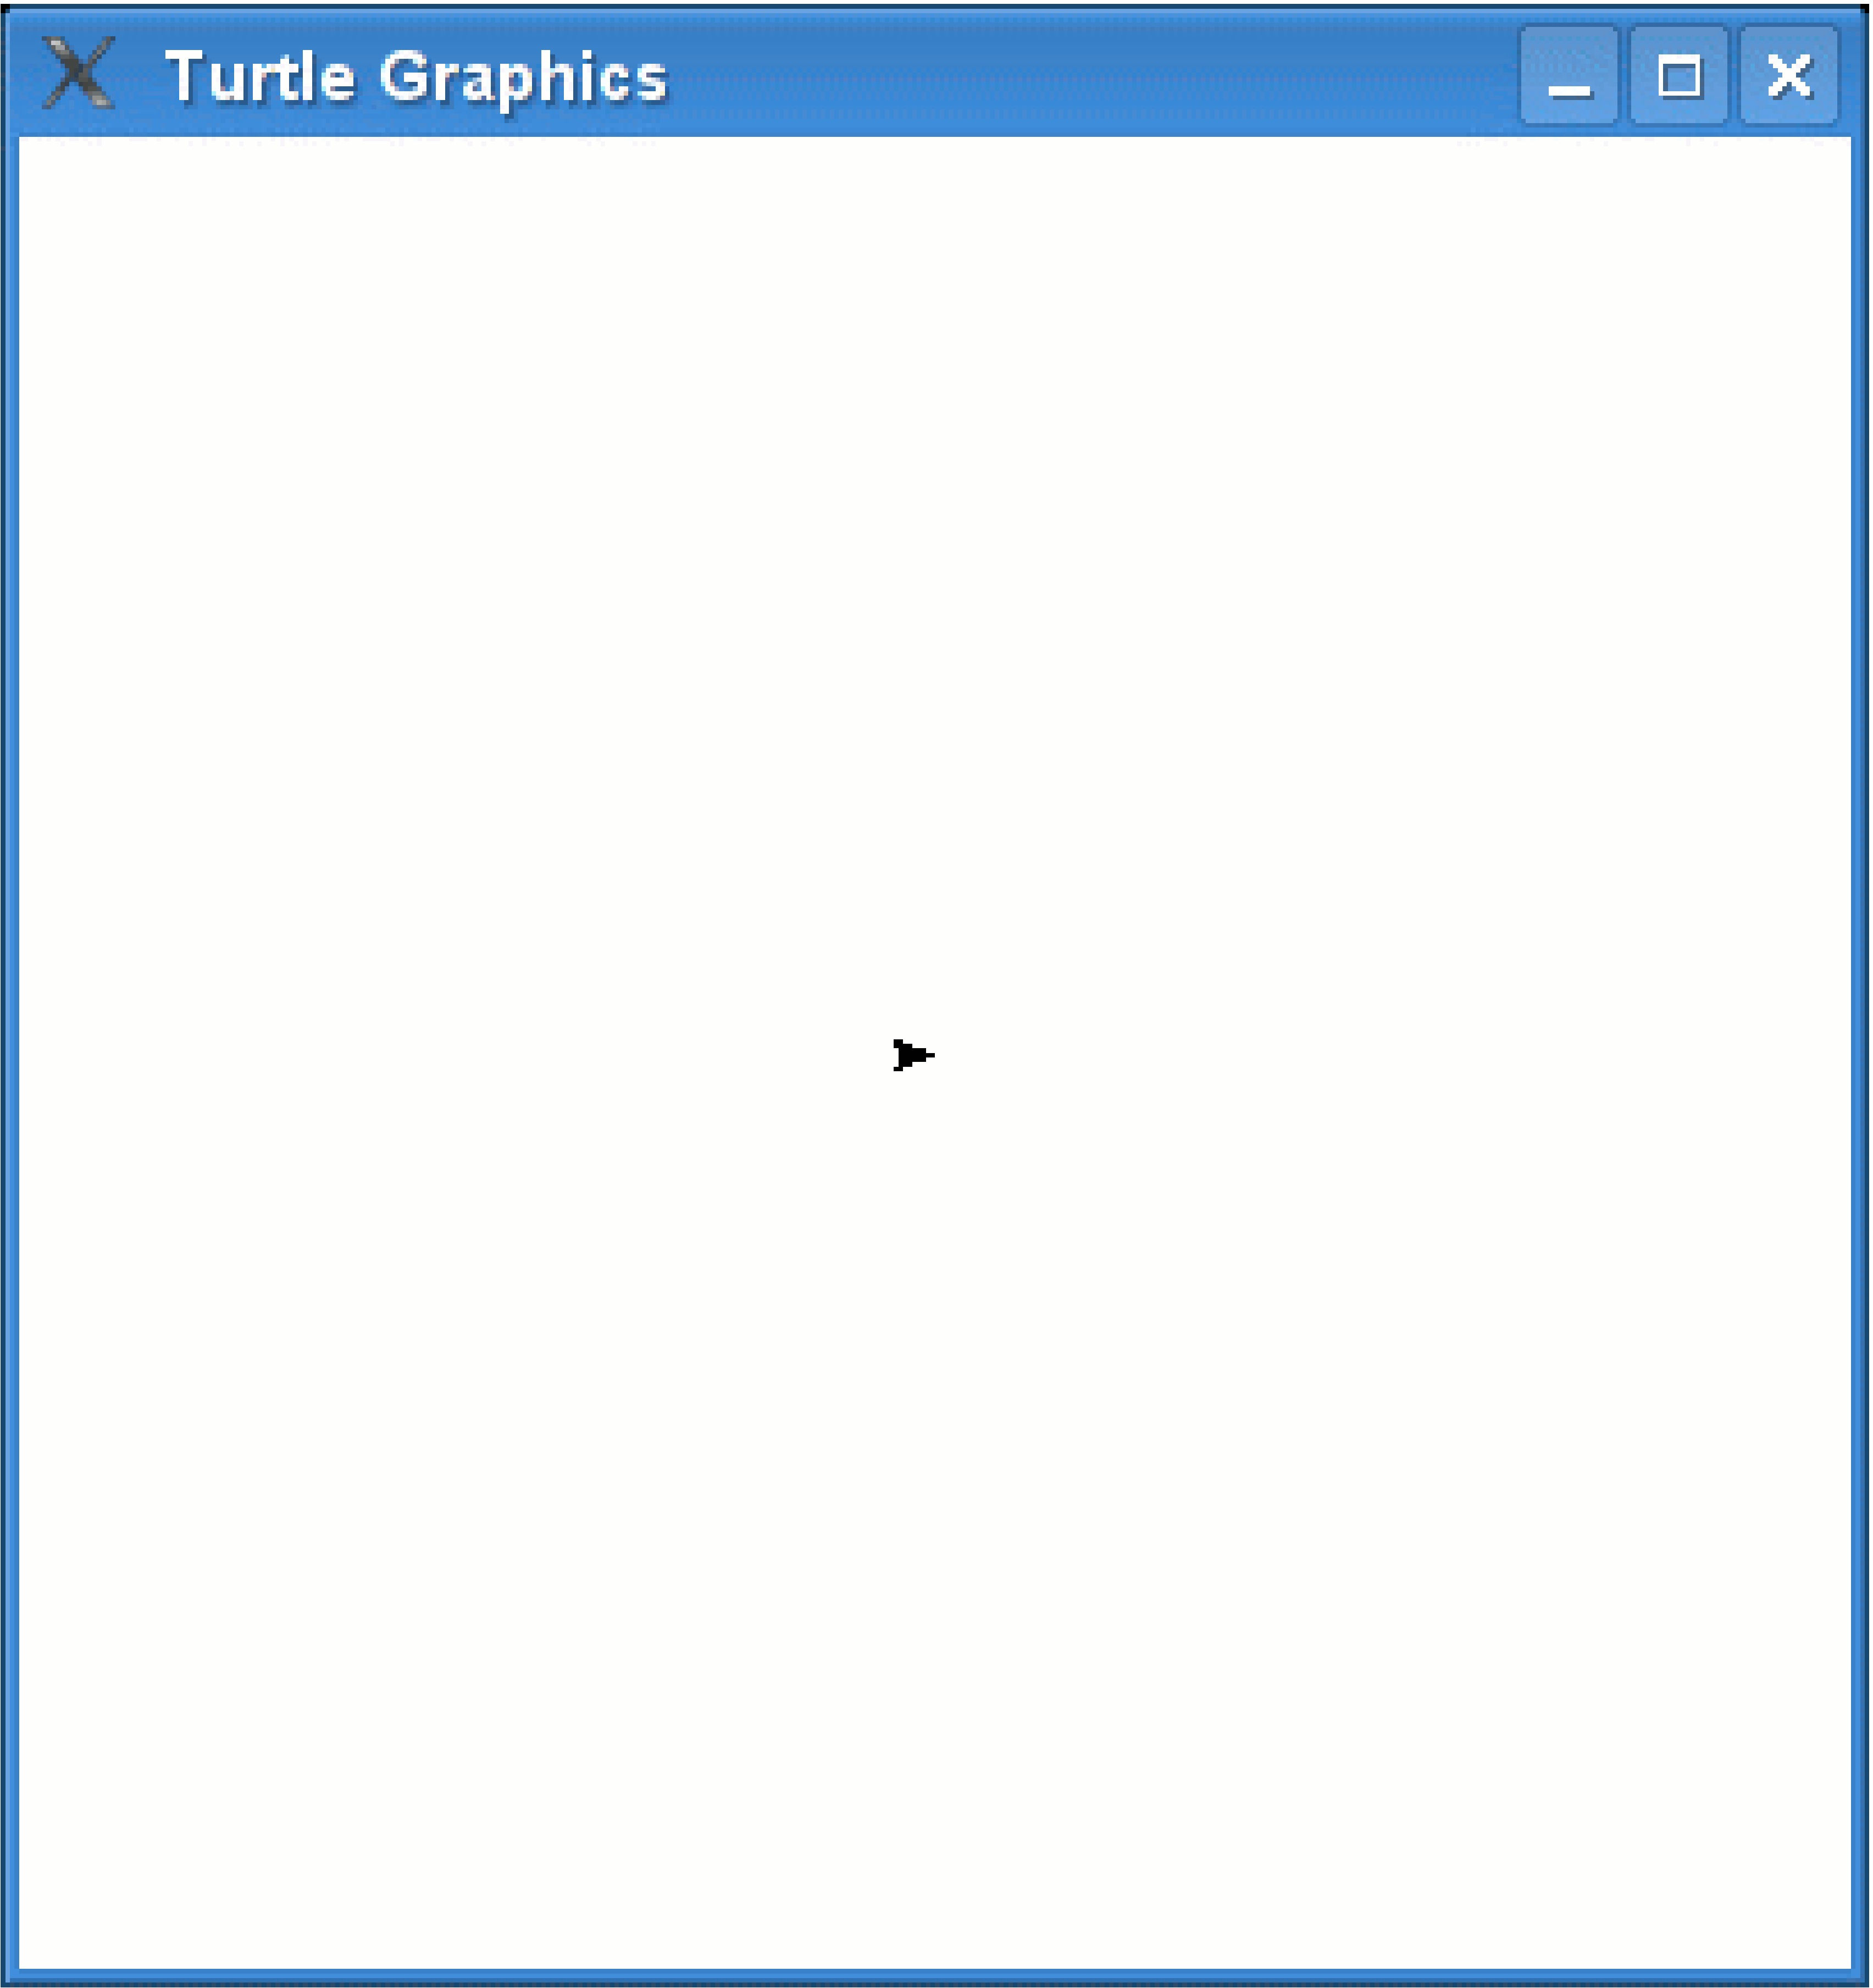
\includegraphics[width=72mm]{images/figure10}
\end{center}
%\caption{An arrow representing the turtle.}\label{fig10}
\caption{Ein Pfeil, der die Schildkröte darstellt.}\label{fig10}
\end{figure}

%\emph{Yes, that little arrow in the middle of the screen really is the turtle.  And, no, it's not very turtle-like.}
\emph{Ja, dieser kleine Pfeil in der Mitte des Bildschirmes ist wirklich die Schildkröte. Und ja, ich weiß, sie schaut nicht besonders sehr nach einer Schildkröte aus.}


%You can send instructions to the turtle, by using functions on the object that was created (by calling \code{turtle.Pen})---since we assigned that object to the variable \code{t}, we use \code{t} to send the instructions.
Jetzt kannst du Befehle an die Schildkröte schicken, indem zu Funktionen auf das Objekt anwendest, das beim \code{turtle.Pen} Aufruf zurückkam. Nachdem wir das Objekt `schildkroete' genannt haben, können wir unsere Befehle an \code{schildkroete} schicken.
%One turtle instruction is \code{forward}.  Forward\index{turtle!forward} tells the turtle to move forward in whatever direction she is facing (I have no idea whether it's a boy or a girl turtle, but let's just assume it's a girl-turtle for the moment). Let's tell the turtle to move forward 50 pixels (we'll talk about pixels in a minute):
Eine Funktion ist  \code{forward}. Forward\index{Schildkröte!vorwärts} bedeutet vorwärts und sagt der Schildkröte sich nach vorne (wohin ihre Nase zeigt) zu bewegen. Lass uns der Schildkröte sagen, dass sie sich 50 Pixel nach vorne bewegen soll (Pixel werden gleich erklärt).

%\begin{listing}
%\begin{verbatim}
%>>> t.forward(50)
%\end{verbatim}
%\end{listing}
\begin{Verbatim}[frame=single]
>>> schildkroete.forward(50)
\end{Verbatim}

%You should see something like figure~\ref{fig11}.
Es sollte etwas wie in Abbildung~\ref{fig11} erscheinen.

\begin{figure}
\begin{center}
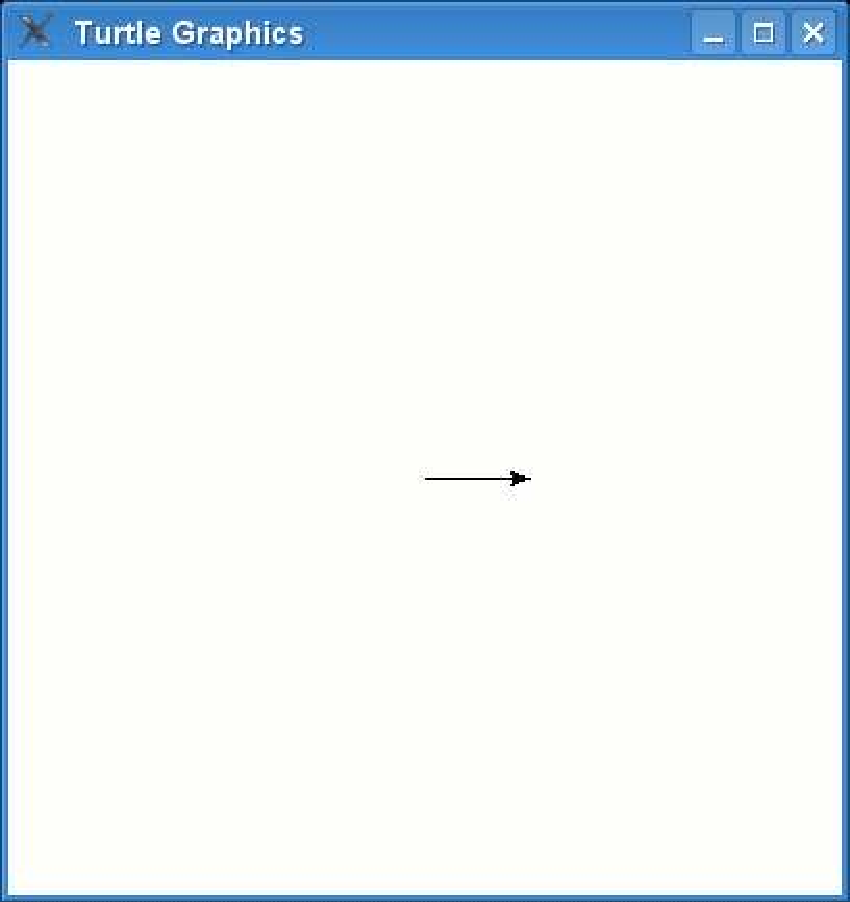
\includegraphics[width=72mm]{images/figure11}
\end{center}
%\caption{The turtle draws a line.}\label{fig11}
\caption{Die Schildkröte zeichnet eine Linie.}\label{fig11}
\end{figure}

%From the turtle's point-of-view, she has moved forward 50 steps.  From our point-of-view, she has moved 50 pixels.
Aus ihrer Sicht hat sich die Schildkröte 50 Schritte bewegt. Aus unserer Sicht 50 Pixel

\noindent
%\emph{So, what's a pixel?}
\emph{Was ist also ein Pixel?}

%A pixel\index{pixels} is a dot on the screen.  When you look at your computer, everything is made up of tiny (square) dots.  The programs you use and the games you play on the computer, or with a Playstation, or an Xbox, or a Wii; are all made up of a whole bunch of different coloured dots, arranged on the screen.  In fact, if you look at your computer screen with a magnifying glass, you might just be able to make out some of those dots. So if we zoom in on the canvas and the line that was just drawn by the turtle, we can see the arrow representing the turtle, is also just a bunch of square dots, as you can see in figure~\ref{fig12}.
Ein Pixel\index{Pixel} ist ein Punkt auf dem Bildschirm. Wenn du ganz nah zum Monitor hingehst, erkennst du, dass alles aus winzigen rechteckigen Punkten besteht. Die Programme die du verwendest und Spiele die du auf Playstation, Xbox oder Wii spielst, bestehen auch aus einer Unzahl von bunten Punkten, die am Bildschirm angeordnet sind. Mit der Lupe wirst du vielleicht die einzelnen Punkte noch besser erkennen. Wenn wir die Python Leinwand mit der Schildkröte näher unter die Lupe nehmen, erkennen wir die einzelnen Punkte so wie in Abbildung~\ref{fig12}.

\begin{figure}
\begin{center}
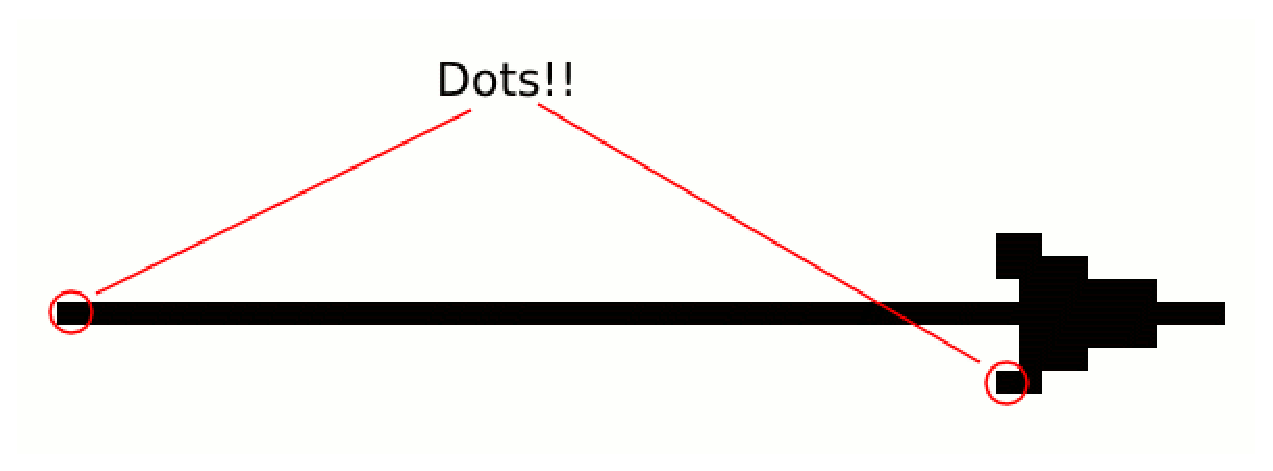
\includegraphics[width=72mm]{images/figure12}
\end{center}
%\caption{Zooming in on the line and the arrow.}\label{fig12}
\caption{Die Linie und das Dreieck näher betrachtet.}\label{fig12}
\end{figure}

%We'll talk more about these dots, or pixels, in a later chapter.
In einem späteren Kapitel werden wir mehr über diese Punkte und Pixel erfahren.

%Next, we can tell the turtle to turn left\index{turtle!turning left} or right\index{turtle!turning right}:
Nun können wir der Schildkröte sagen dass sie links\index{Schildkröte!links abbiegen} oder rechts \index{Schildkröte!rechts abbiegen} abbiegen soll:

%\begin{listing}
%\begin{verbatim}
%>>> t.left(90)
%\end{verbatim}
%\end{listing}
\begin{Verbatim}[frame=single]
>>> schildkroete.left(90)
\end{Verbatim}

%This tells the turtle to turn left, 90 degrees.  You may not have learned about degrees\index{degrees} in school so far, but the easiest way to think about them, is that they are like the divisions on the face of a clock as seen in figure~\ref{fig13}.
Damit sagst du der Schildkröte, dass sie links abbiegen soll (90 Grad). Du hast in der Schule vielleicht schon etwas über Winkelgrad\index{Winkelgrad} gehört. Wenn nicht, könntest du dir das ungefähr wie das Ziffernblatt von einer Uhr vorstellen. Schau mal Abbildung~\ref{fig13} an.

\begin{figure}
\begin{center}
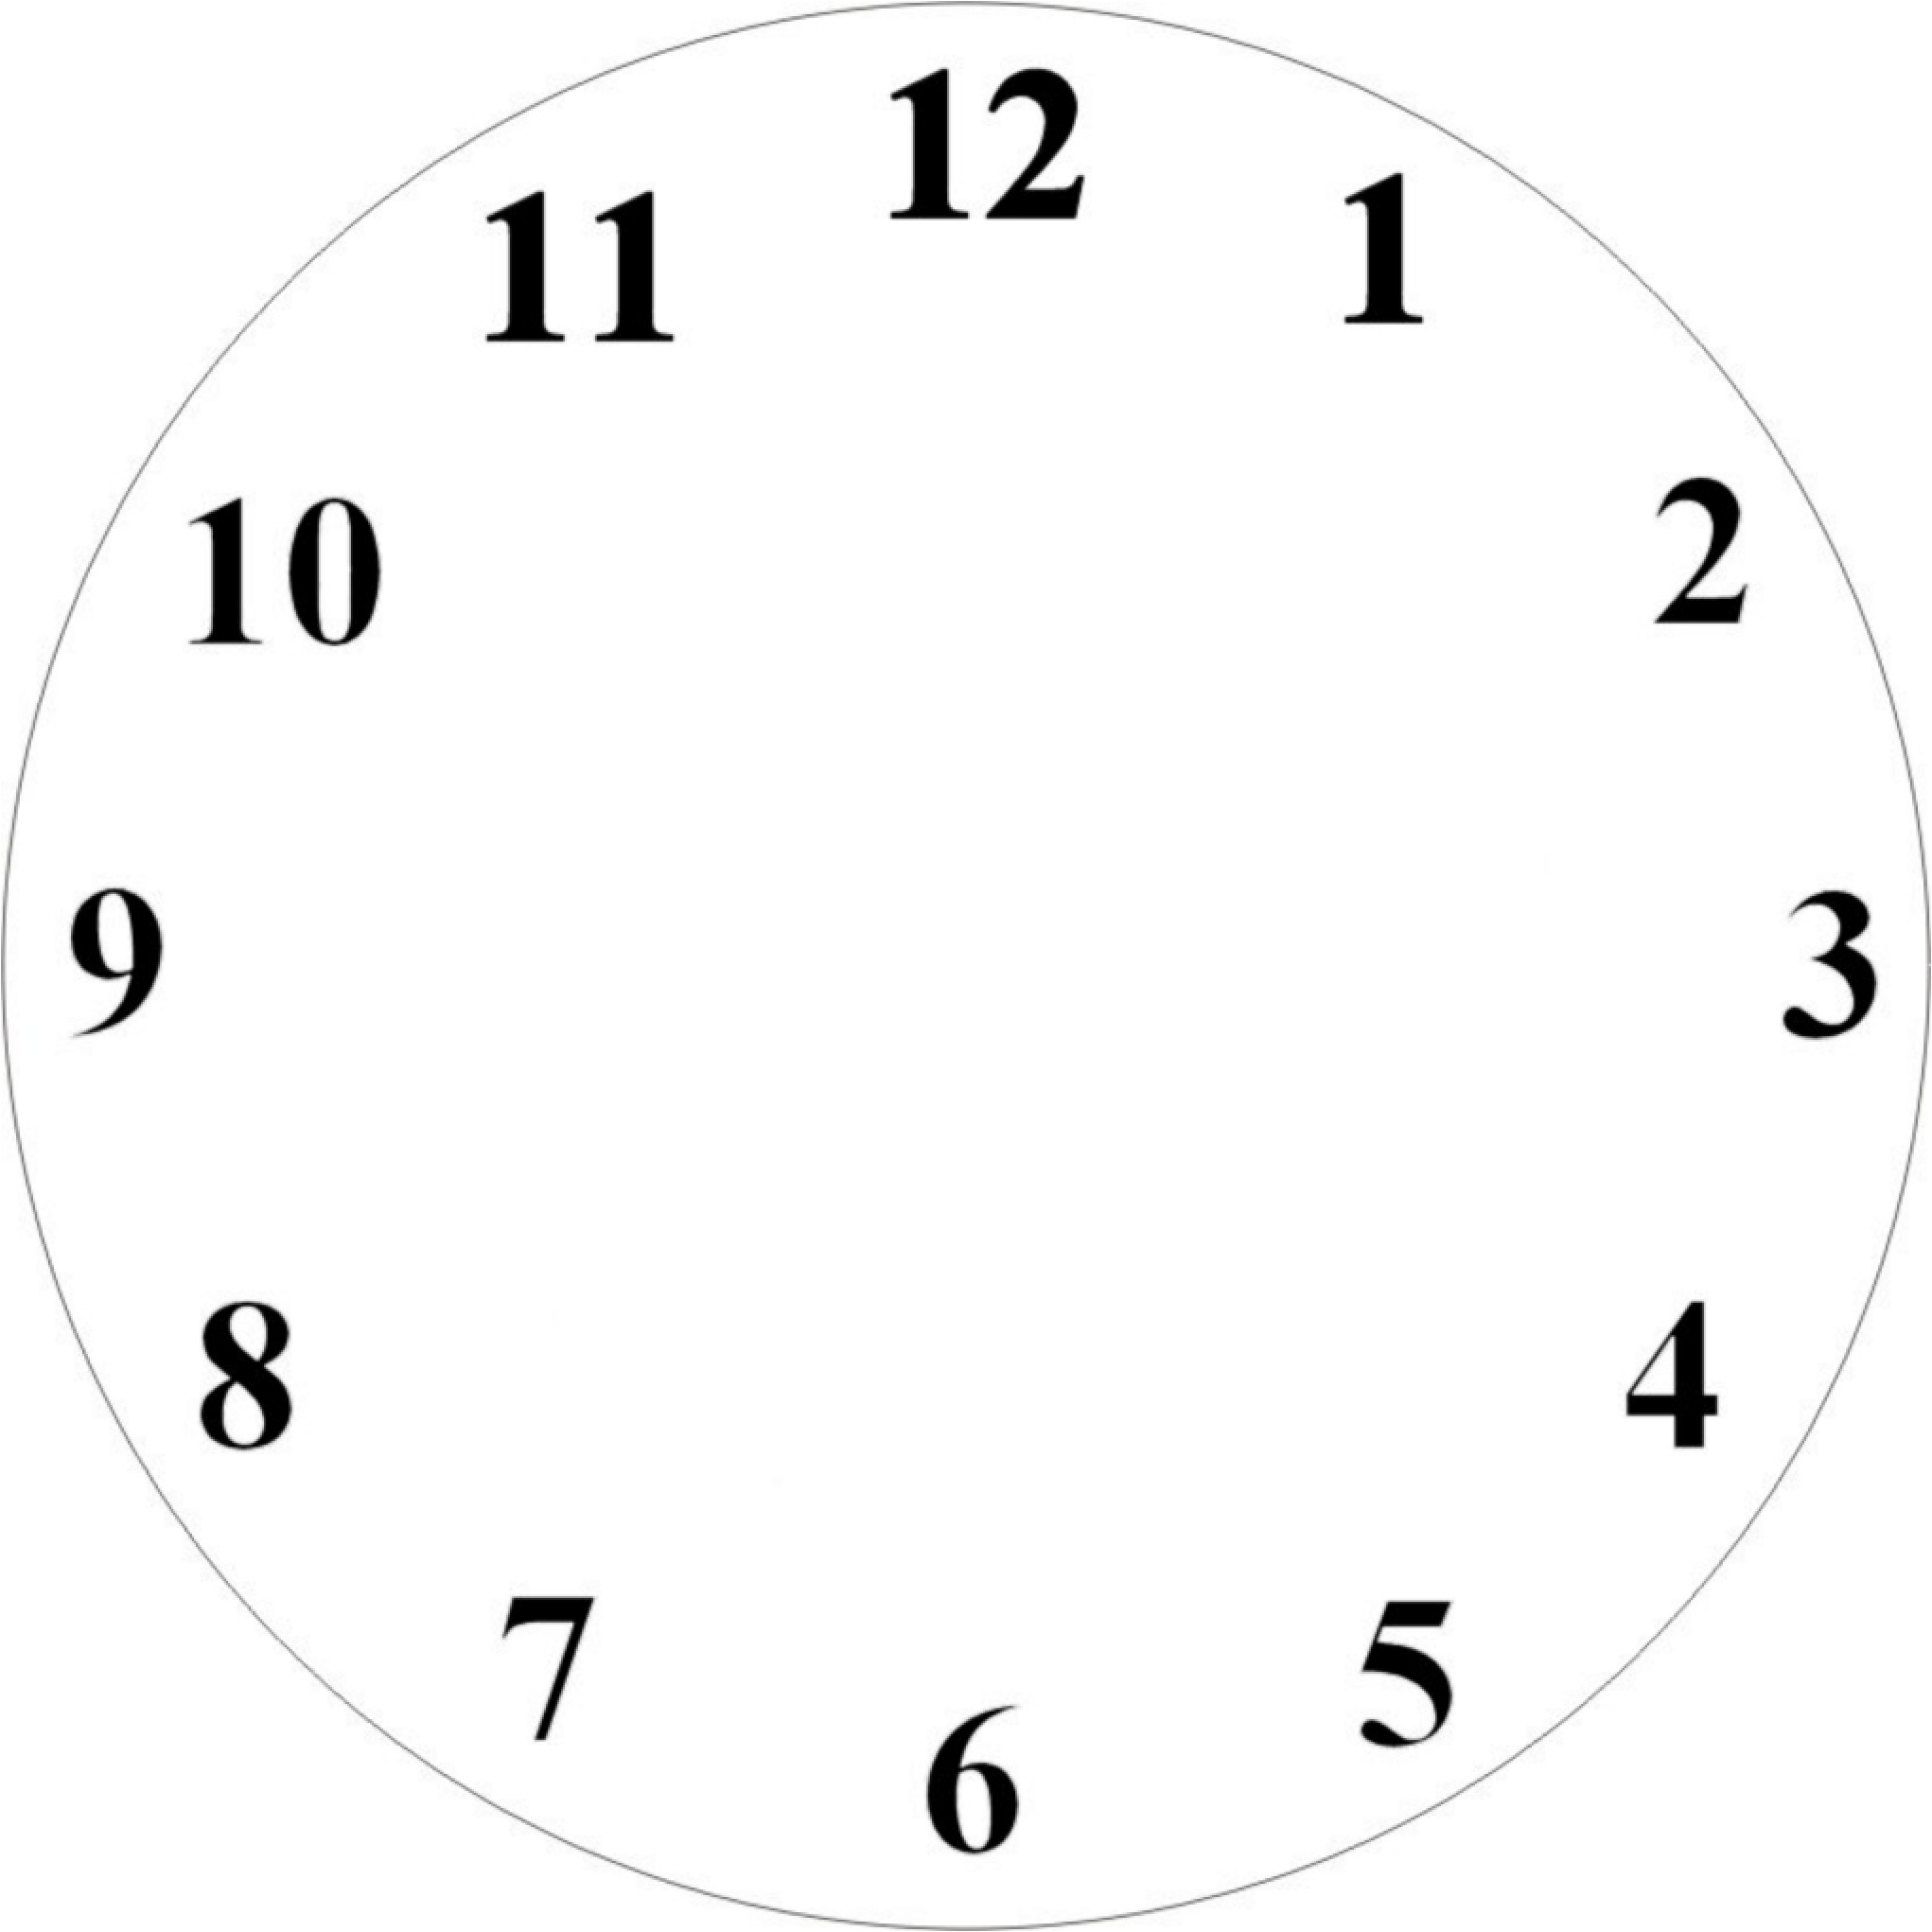
\includegraphics[width=52mm]{images/figure13}
\end{center}
%\caption{The `divisions' on a clock.}\label{fig13}
\caption{Die `Unterteilung' der Uhr.}\label{fig13}
\end{figure}

%The difference to a clock, is that rather than 12 divisions (or 60, if you're counting minutes rather than hours), there are 360 divisions.  So, if you count 360 divisions around the face of a clock, you get 90 where there's normally a 3, 180 where there's normally a 6, and 270 where there's normally a 9; and 0 would be at the top (at the start), where you normally see a 12.  Figure~\ref{fig14} shows you the degree divisions.
Im Unterschied zu einer Uhr, die 12 Unterteilungen hat (oder 60 wenn du die Minuten meinst), gibt es auch die Unterteilung in Grad. Dabei hat eine Umdrehung 360 Grad. Wo bei der Uhr die Unterteilung für 3 Uhr ist, würden es 90 Grad sein. Und bei 6 Uhr sind 180 Grad. In Abbildung~\ref{fig14} siehst du die Unterteilung in Grad.

\begin{figure}
\begin{center}
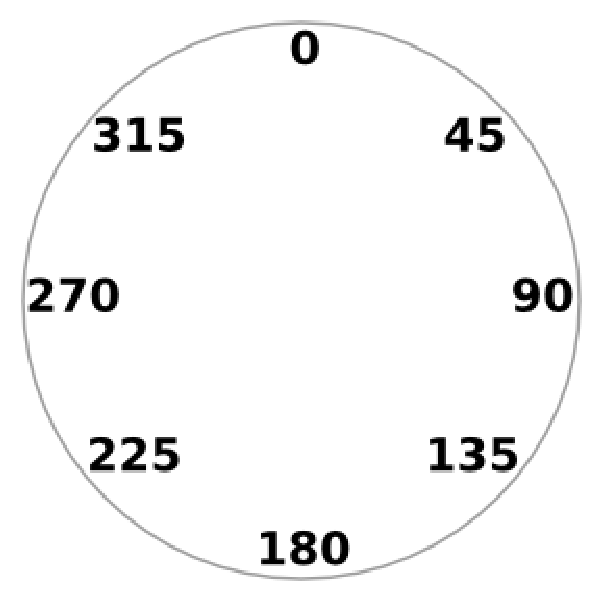
\includegraphics[width=52mm]{images/figure14}
\end{center}
%\caption{Degrees.}\label{fig14}
\caption{Unterteilung des Kreises in Grad.}\label{fig14}
\end{figure}


%So, what does it actually mean when you call \code{left(90)}?
Was heißt das also genau, wenn wir \code{left(90)} schreiben?
\par
%If you stand and face one direction, point your arm out directly away from your shoulder, THAT is 90 degrees.  If you point your left arm, that's 90 degrees left.  If you point your right arm, that's 90 degrees right.  When Python's turtle turns left, she plants her nose in one spot then swivels her body around the face the new direction (same as if you turned your body to face where your arm is pointing).  So, \code{t.left(90)} results in the arrow now pointing upwards, as shown in figure~\ref{fig15}.
Wenn du aufrecht stehst und deinen Arm seitlich ausstreckst, dann sind das genau 90 Grad. Wenn du den linken Arm ausstreckst, sind das 90 Grad links und wenn du den rechten Arm ausstreckst, sind das 90 Grad rechts. Wenn die Python Schildkröte links abbiegt, dann dreht sie sich um 90 Grad links. Das ist das gleiche, wie wenn du deinen Körper so herumdrehst, dass du danach in die Richtung deiner ausgestreckten Hand schaust. Nachdem du also \code{schildkroete.links(90)} eingegeben hast, zeigt die Schildkröte nach oben wie du es in Abbildung~\ref{fig15} sehen kannst.

\begin{figure}
\begin{center}
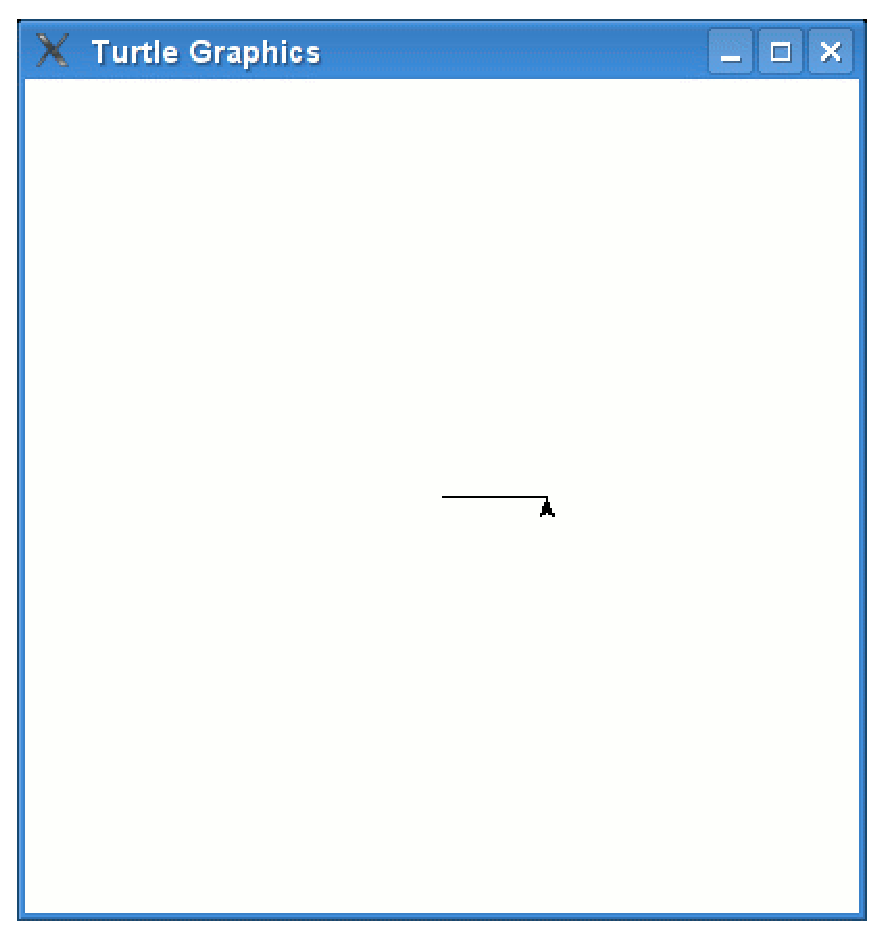
\includegraphics[width=72mm]{images/figure15}
\end{center}
%\caption{The turtle after turning left.}\label{fig15}
\caption{Die Schildkröte nachdem sie links abgebogen ist.}\label{fig15}
\end{figure}

%Let's try the same commands again a few times:
Probieren wir das noch einmal:

%\begin{listing}
%\begin{verbatim}
%>>> t.forward(50)
%>>> t.left(90)
%>>> t.forward(50)
%>>> t.left(90)
%>>> t.forward(50)
%>>> t.left(90)
%\end{verbatim}
%\end{listing}
\begin{Verbatim}[frame=single]
>>> schildkroete.forward(50)
>>> schildkroete.left(90)
>>> schildkroete.forward(50)
>>> schildkroete.left(90)
>>> schildkroete.forward(50)
>>> schildkroete.left(90)
\end{Verbatim}

%Our turtle has drawn a square and is left facing the same direction as she started (see figure~\ref{fig16}).
Unsere Schildkröte hat ein Quadrat gezeichnet und schaut wieder in die selbe Richtung, wie sie gestartet ist (schau dir Abbildung~\ref{fig16} an).

\begin{figure}
\begin{center}
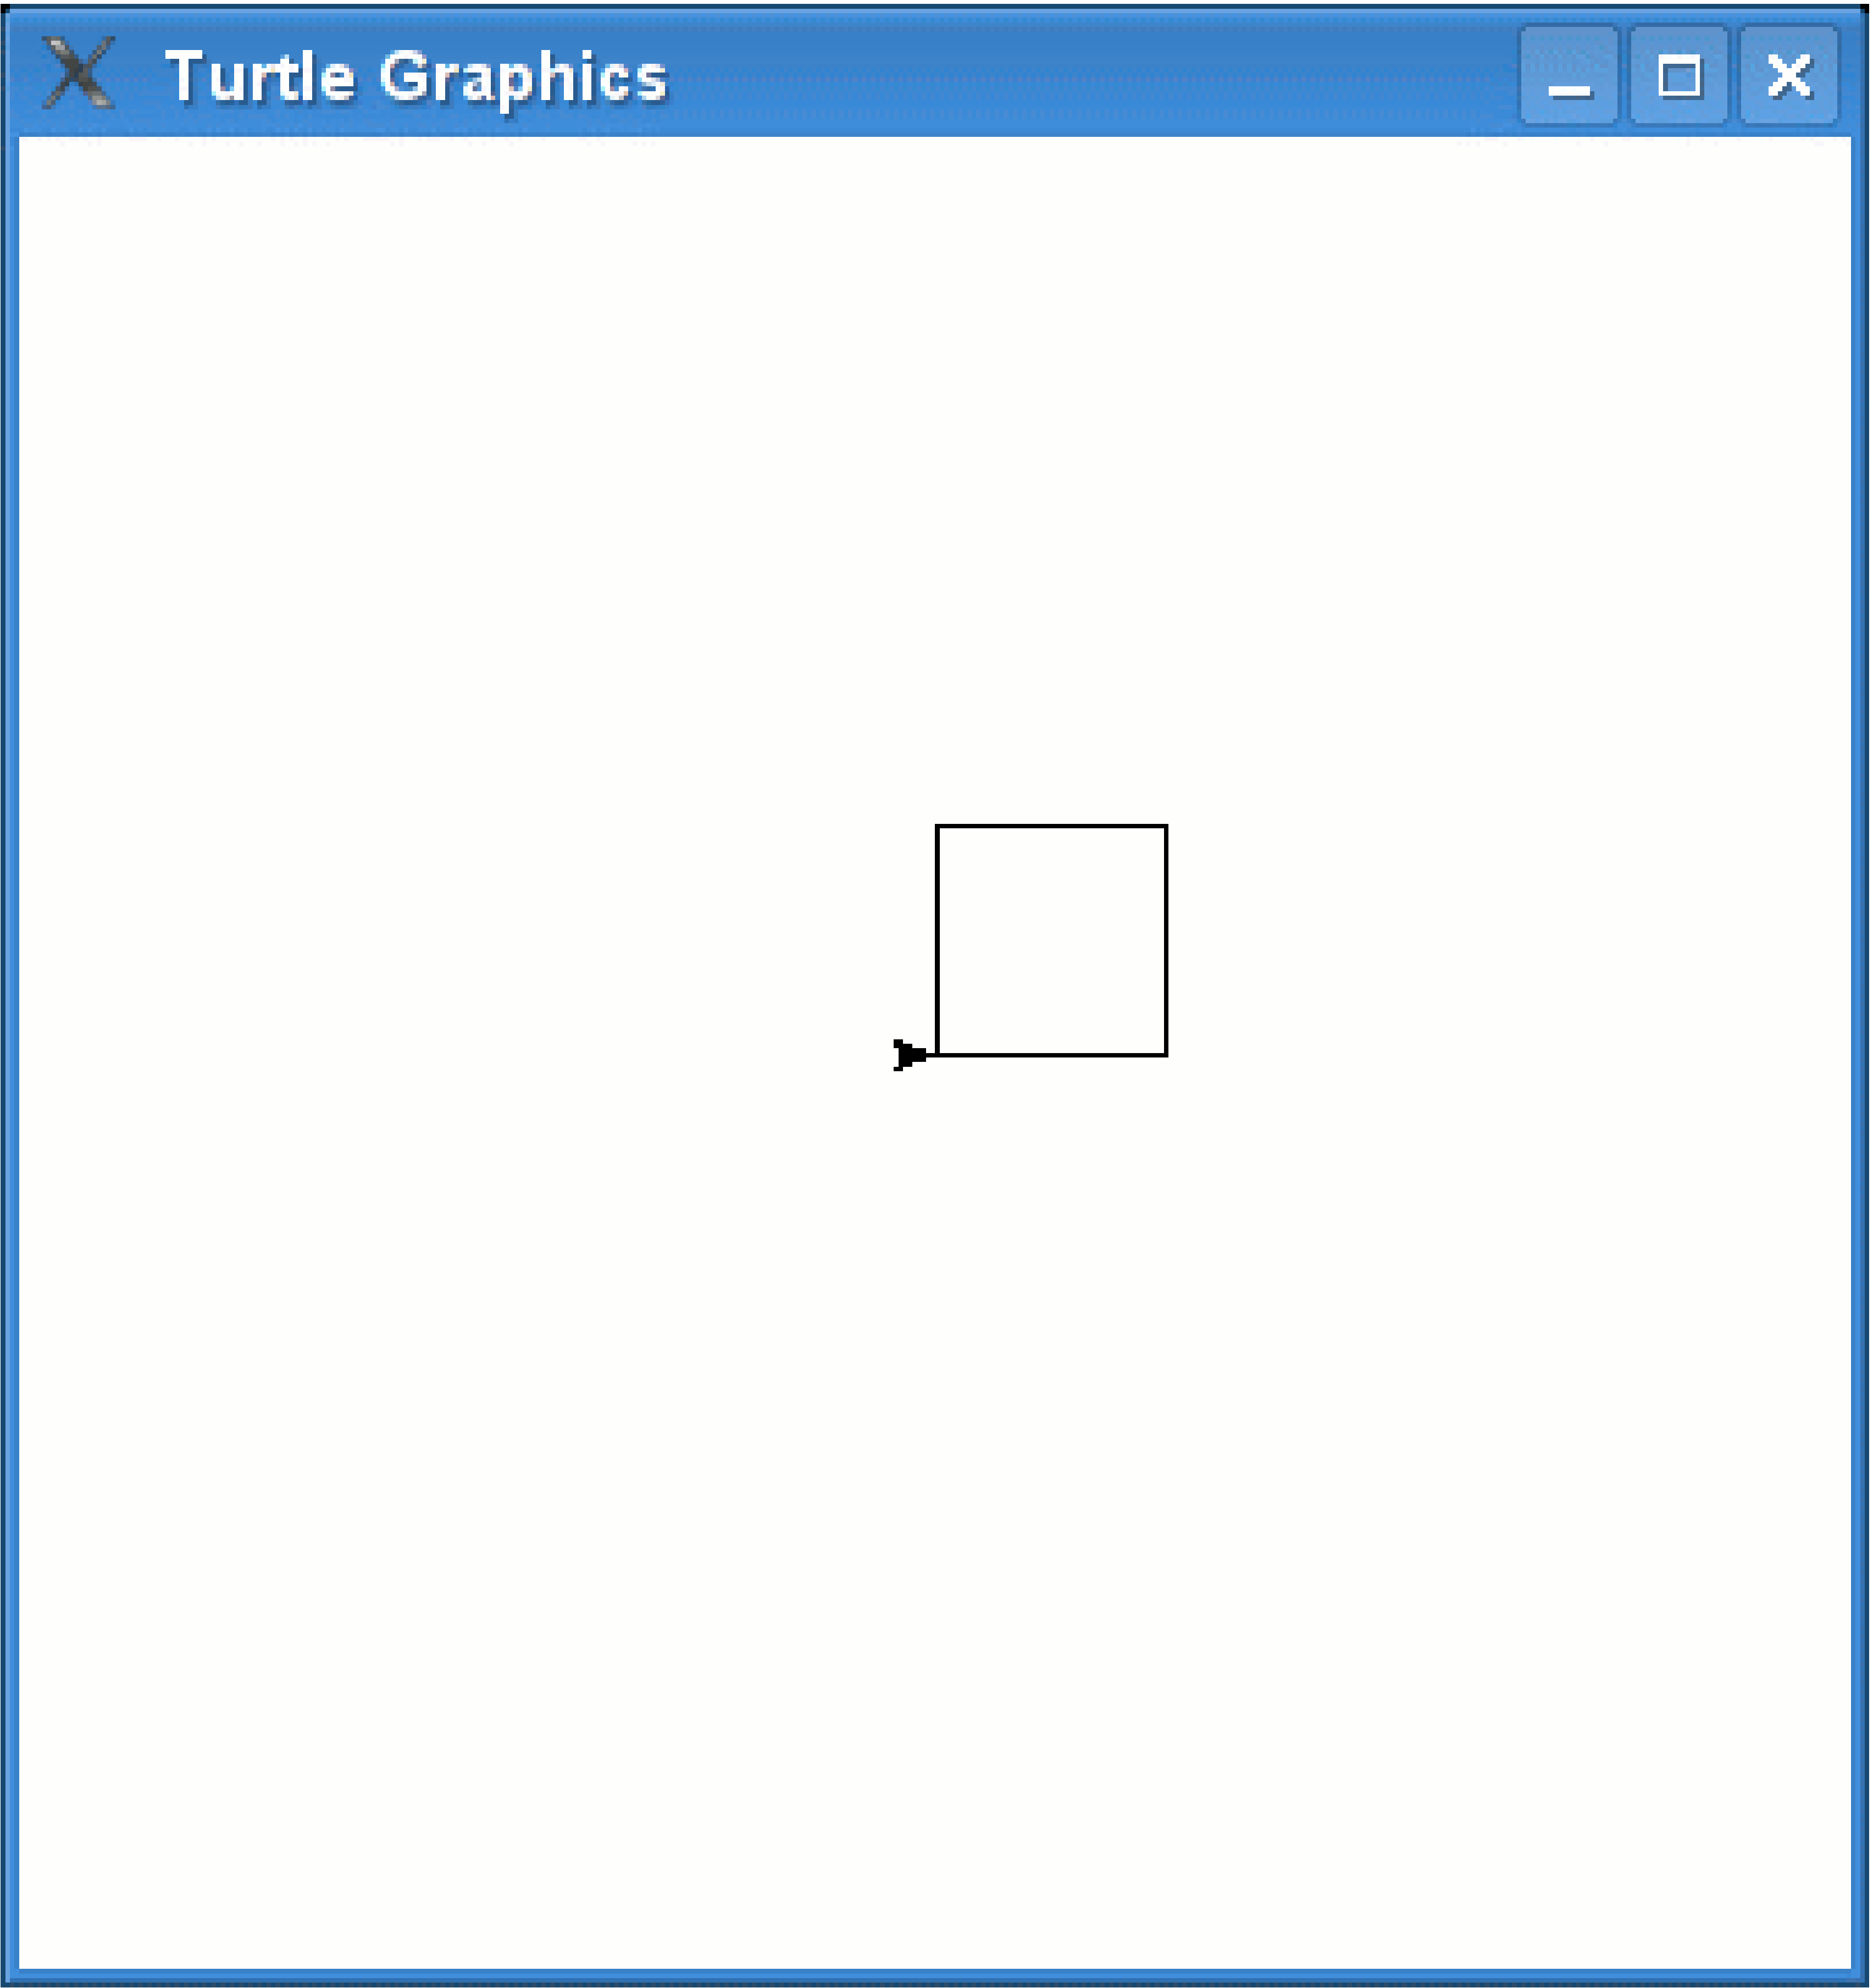
\includegraphics[width=72mm]{images/figure16}
\end{center}
%\caption{Drawing a square.}\label{fig16}
\caption{Ein Quadrat zeichnen.}\label{fig16}
\end{figure}

%We can erase what's on the canvas by using clear\index{turtle!clear}:
Wir können die Leinwand auch löschen, indem wir den Befehl clear\index{Schildkröte!Leinwand löschen} aufrufen:

%\begin{listing}
%\begin{verbatim}
%>>> t.clear()
%\end{verbatim}
%\end{listing}
\begin{Verbatim}[frame=single]
>>> schildkroete.clear()
\end{Verbatim}

%Some of the other basic functions you can use with your turtle are: \code{reset}\index{turtle!reset}, which also clears the screen, but puts the turtle automatically back into her starting position; \code{backward}\index{turtle!backward}, which moves the turtle backwards; \code{right}, which turns the turtle to the right; \code{up}\index{turtle!up (stop drawing)} which tells the turtle to stop drawing as she moves (in other words pick her pen up off the canvas); and finally \code{down}\index{turtle!down (start drawing)} which tells the turtle to start drawing again. You call these functions in the same way we've used the others:
Einige andere Befehle, die die Schildkröte versteht sind: \code{reset}\index{Schildkröte!zurücksetzen} was auch die Leinwand löscht, aber die Schildkröte auch wieder am Start absetzt; mit \code{backward}\index{Schildkröte!rückwärts} geht die Schildkröte rückwärts; mit \code{right}\index{Schildkröte!rechts} biegt die Schildkröte rechts ab; und wenn sie keine Spur mehr zeichnen soll, dann gibt man \code{up}\index{Schildkröte!up (aufhören zu zeichnen)} ein. Wenn die Schildkröte wieder zeichnen anfangen soll, dann gib \code{down}\index{Schildkröte!down (anfangen zeichnen)} ein. Du kannst diese Befehle wie gewohnt verwenden:

%\begin{listing}
%\begin{verbatim}
%>>> t.reset()
%>>> t.backward(100)
%>>> t.right(90)
%>>> t.up()
%>>> t.down()
%\end{verbatim}
%\end{listing}
\begin{Verbatim}[frame=single]
>>> schildkroete.reset()
>>> schildkroete.backward(100)
>>> schildkroete.right(90)
>>> schildkroete.up()
>>> schildkroete.down()
\end{Verbatim}

\noindent
%We'll come back to the turtle module shortly.
Wir kommen später wieder auf das Schildkröten Modul zurück.

%\section{Things to try}
\section{Probiere es aus}

%\emph{In this chapter we saw how to use turtle to draw simple lines, using left and right turns.  We saw that turtle uses degrees to turn, a bit like the minute divisions on a clock face.}
\emph{In diesem Kapitel haben wir gesehen, wie mit dem Turtle Modul einfache Linien gezeichnet werden. Wir haben auch Gradangaben verwendet, wenn die Schildkröte in eine andere Richtung zeigen soll.}

%\subsection*{Exercise 1}
\subsection*{Übung 1}
%Create a canvas using turtle's \code{Pen} function, and draw a rectangle.
Erzeuge eine Leinwand indem du die turtle Funktion \code{Pen} verwendest und zeichne ein Rechteck.

%\subsection*{Exercise 2}
\subsection*{Übung 2}
%Create another canvas using turtles \code{Pen} function, and draw a triangle.
Erzeuge wieder eine Leinwand indem du die Funktion \code{Pen} aufrufst und zeichne ein Dreieck.

\newpage
